% Chapter 5

\chapter{Trying to improve the State of the Art}

\lhead{Chapter 5. \emph{Trying to improve the State of the Art}} % This is for the header on each page - perhaps a shortened title
\label{chp:refwork}
%----------------------------------------------------------------------------------------

\def\:{\hskip0pt} %Definisce un modo veloce per permettere a latex di sillabare correttamente anche parole come 4-connectivity. Il corretto utilizzo è il seguente: 4\:-\:connectivity.
The architecture proposed by Cipriano et al. was quite simple yet effective. The
main novel addition was the use of positional encoding. We now want to try to
improve the results obtained by them by adding some more complex
and more recent architectures, losses, and optimizers.

\section{Boundary Loss}
Jointly with PosPadUNet3D, standard DICE loss was used. We also tried to use
CrossEntropy loss, but the results were not as good as with DICE loss so it has
been discarded. As we were dealing with highly unbalanced data, less than 1\% of
the whole volume is the canal, we looked for alternative losses which deal with
this problem.

Kervadec et al. \cite{kervadec2019boundary} proposed a loss function that takes
the form of a distance metric on the space of contours instead of regions. Dice
or cross-entropy, are based on regional integrals, which are convenient for
training deep neural networks. In practice, these regional integrals are
summations over the segmentation regions of differentiable functions, each
directly invoking the softmax probability outputs of the network. Therefore,
standard stochastic optimizers such as SGD are directly applicable.
Unfortunately, difficulties occur for highly unbalanced segmentations, for
instance, when the size of the target foreground region is several orders of
magnitude less than the background size, which is a common characteristic for
medical images. The problem with such losses is that they assume identical
importance distribution for all the samples and classes.

In the aforementioned paper, the authors proposed a new type of loss, named
\emph{Boundary loss} that aims to mitigate the issues related to regional losses
in highly unbalanced segmentation problems. Rather than using unbalanced
integrals over the regions, a boundary loss uses integrals over the boundary
between the regions. Furthermore, it provides information that is complementary
to regional losses. It is, however, challenging to represent the boundary points
corresponding to the regional softmax outputs of a CNN. This difficulty may
explain why boundary losses have been avoided in the context of deep
segmentation networks.

\subsection{Formulation}
The Boundary loss has been formulated as follows: let $I: \Omega \subset
\mathbb{R}^{2,3} \rightarrow \mathbb{R}$ denotes an image with spatial domain
$\Omega$, and $g: \Omega \rightarrow {0,1}$ a binary ground truth segmentation
of the image such that $g(p) = 1$ if the pixel $p$ belongs to the target region
$G \subset \Omega$ and $0$ otherwise. Let $s_\theta : \Omega \rightarrow [0,1]$
denotes the softmax probability output of a deep segmentation network, and
$S_\theta \subset \Omega$ denotes the corresponding segmentation region:
$\S_\theta = {p \in \Omega | s_\theta(p) >= \delta}$ for some threshold
$\delta$. Let $\Delta G$ denote a representation of the boundary of the
ground-truth region $G$ (i.e. the set of points of $G$, which have a spatial
neighbor in background $\Omega \setminus G$) and $\Delta S_\theta$ denoting the
boundary of the segmentation region defined by the network output.\\
The boundary loss can now be defined as:

\begin{equation}
  \label{eq:boundaryloss}
  \mathcal{L}_{\text{boundary}}(\theta) = \int_{\Omega} \phi_G(q)s_\theta(q)dq
\end{equation}

Where $\phi_G$ is the level set of the ground-truth region $G$, obtained by
using the signed distance transform over $G$.

\subsection{Combining with other loss functions}
As we have already said, this type of loss is complementary to the regional
losses, since it provides information about the boundary of the segmentation
region, therefore they can be combined. In our experiments, we used the
following combination:
\begin{equation}
  \label{eq:boundaryloss}
  \mathcal{L}(\theta) = (1-\alpha)\mathcal{L}_{\text{boundary}}(\theta) +
  \alpha\mathcal{L}_{\text{DICE}}(\theta)
\end{equation}
Where $\alpha$ is a hyperparameter that weights the two losses.

Kervadec et al. in the paper where they presented this type of novel loss
they've adopted a peculiar way to set this $\alpha$. As the training was kind of
unstable they set $\alpha$ to an initial value of $0$ and increased its value by
$0.01$ and each training epoch until a fixed threshold. This type of approach
have given the best results in terms of stability and performance thus we
decided to adopt it also in our experiments.

\section{PosDeepLab v3+}
DeepLab v3+ is another well-known architecture for semantic segmentation. It was
proposed by Chen et al. in 2017 with version 1. Later in the years, they
proposed small changes to the architecture, which resulted in version 2, 3, and
the latest one, version 3+. The main novelty that can be found in this
architecture is the use of Atrous Spatial Pyramid Convolutions, which are
dilated convolutions in parallel, each one with a different dilation rate and
later concatenated, the use of a fully connected Conditional Random Field, which
improves the segmentation by maximizing the label agreement between similar
pixels, and the use of depth-wise separable convolutions, which are a way to
reduce the number of parameters in the network. The model architecture is shown
in Figure \ref{fig:deeplabv3+}.
\begin{figure}[h]
  \centering
  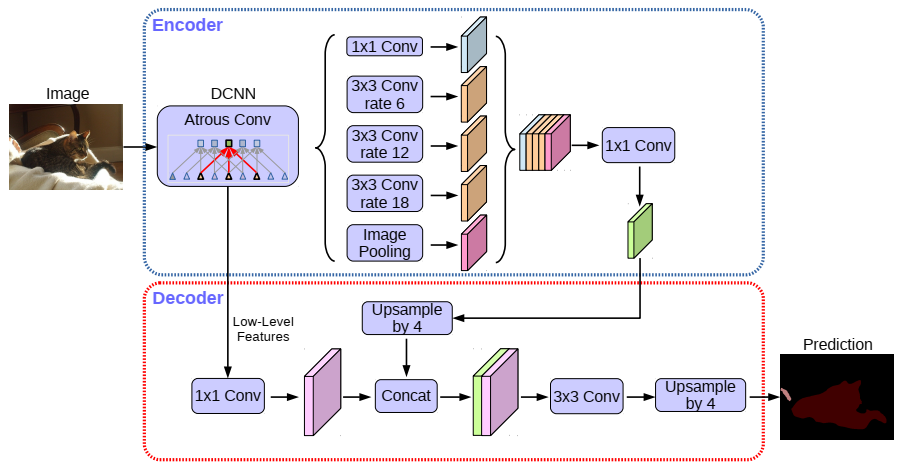
\includegraphics[width=0.8\textwidth]{Images/DeepLabv3+.png}
  \caption{DeepLab v3+ architecture}
  \label{fig:deeplabv3+}
\end{figure}

\section{PosSegNet}
SegNet is a fully convolutional network for semantic segmentation. It was
proposed by Badrinarayanan et al. in 2015 and is structured in two parts: an
encoder and a decoder, similar to the one used in the U-Net. While the encoder
is made of convolutional layers followed by max pooling. The indices of the
max pooling are stored to be used in the decoder during the upsampling.
The encoder part is made of the 13 convolutional layers of the VGG16 network,
while in the decoder always 13 layers are used, but they are made of transposed
convolutional layers. Finally, a K-class softmax classifier is used to predict
the class for each pixel.
Also in this case the same positional encoding used in PosPadUNet3D was
introduced, as it was shown to be effective in the previous architecture.
SegNet was originally proposed for the segmentation of images, but by changing
the 2D operations to 3D ones, it can be used for the segmentation of 3D volumes.
The architecture is shown in figure \ref{fig:segnet}.
\begin{figure}[h]
  \centering
  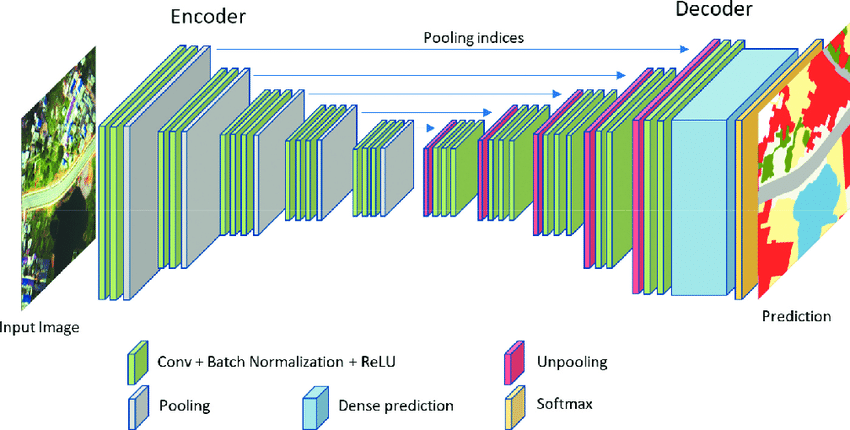
\includegraphics[width=0.5\textwidth]{Images/segnet.png}
  \caption{SegNet architecture}
  \label{fig:segnet}
\end{figure}

\section{SwinUNETR3D}
Hatamizadeh et al. recently proposed a novel architecture for 3D medical image
segmentation which make use of the Transformer architecture. The main idea is to
replace the convolutions of U-Net used in the encoding phase with Transformers.
Instead of the standard Vision Transformers, Swin Transformers have been used as
they have shown better performance on images. As Transformers are known to
suffer where there is a lack of data, also a pre-training procedure has been
proposed to overcome this problem. In the following sections, we will describe
the proposed architecture, starting from the standard Transformer as proposed in
the original paper "Attention is all you need" by Vaswani et al., and then we
will look at how these ideas have been moved from NLP to Computer Vision.

\subsection{Transformer Architecture}
The transformer architecture was first introduced by Vaswani et al. in $2017$ in
the field of Natural Language Processing. The main idea is to replace a
recurrent layer with a multi-head attention mechanism, which is a linear
operation that can be computed in parallel.
The attention mechanism is computed as follows:
\begin{equation}
  \label{eq:attention}
  \text{Attention}(Q,K,V) = \text{softmax}(\frac{QK^T}{\sqrt{d_k}})V
\end{equation}
Where $Q \in \mathbb{R}^{d_k}$ is the query, $K \in \mathbb{R}^{d_k}$ is the key
and $V \in \mathbb{R}^{d_v}$ is the value. If we would like to make it
multi-head, we add more attention layers in parallel and concatenate the
results. The final output of a multi-head attention layer is computed as
follows:
\begin{equation}
  \label{eq:multiheadattention}
  \text{MultiHeadAttention}(Q,K,V) = \text{Concat}(\text{head}_1, \dots,
  \text{head}_h)W^O
\end{equation}
where $\text{head}_i = \text{Attention}(QW_i^Q, KW_i^K, VW_i^V)$.
The projection matrices $W_i^Q \in \mathbb{R}^{d_{\text{model}} \times d_k}$,
$W_i^K \in \mathbb{R}^{d_{\text{model}} \times d_k}$, $W_i^V \in
\mathbb{R}^{d_{\text{model}} \times d_v}$, and $W^O \in \mathbb{R}^{hd_v \times
d_\text{model}}$ are learned parameters. The complete architecture, which also
adds a residual connection, a linear layer, and a normalization layer, is shown
in Figure \ref{fig:transformer}.
\begin{figure}[h]
  \centering
  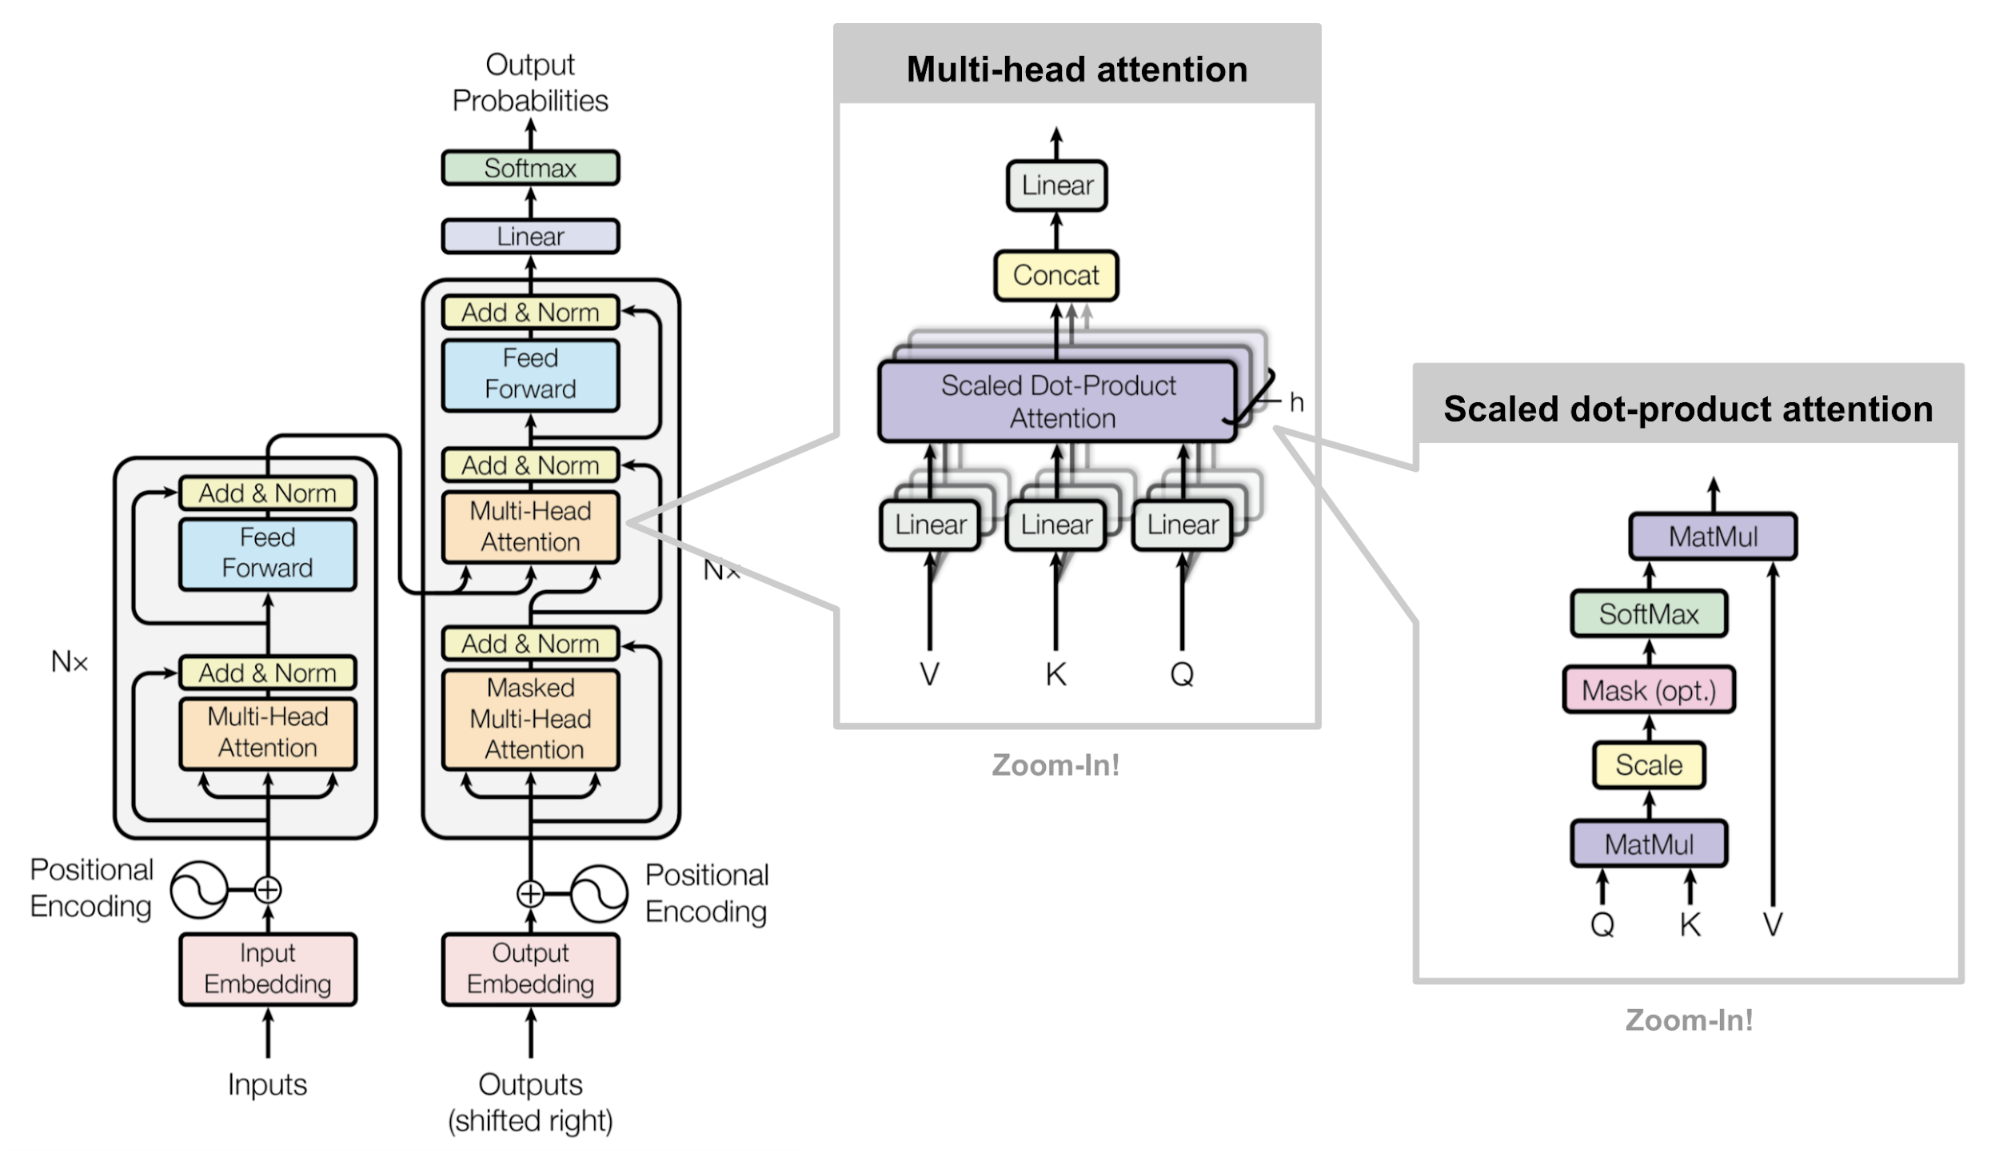
\includegraphics[width=0.8\textwidth]{transformer.png}
  \caption{Transformer architecture}
  \label{fig:transformer}
\end{figure}

\subsection{Vision Transformer}
While the Transformer architecture has become the de-facto standard for natural
language processing tasks, its applications to computer vision have remained
limited for a few years. One of the reasons is that the complexity of the
attention mechanism is $O(n^2)$, where $n$ is the number of pixels in the image.
This makes it impractical for medium and large-size images. In $2020$,
Dosovitskiy et al. proposed a novel architecture called Vision Transformer (ViT)
which is able to scale up the Transformer architecture to images. The main idea
is to reshape the original image $x \in \mathbb{R}^{H \times W \times C}$ into a
sequence of patches $x_p \in \mathbb{R}^{P \times P \times C}$, where $H$, $W$,
$C$ and $P$ are the height, width, number of channels and resolution of patches
respectively. The Transformer uses constant latent vector size $D$ through all
of its layers, so we flatten the patches and map to D dimensions with a
trainable linear projection. The outputs of such projections are patch
embeddings. An additional token \texttt{[class]} is added to the sequence, which
is used to encode the class label of the image. The whole architecture is
depicted in Figure \ref{fig:visiontransformer}.

\begin{figure}[ht!]
  \centering
  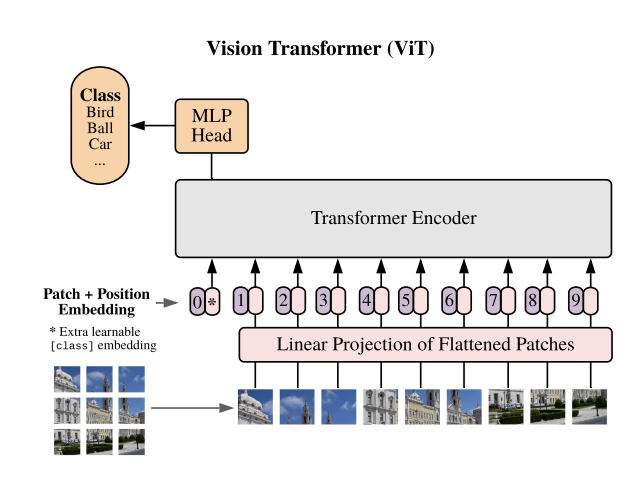
\includegraphics[width=0.5\textwidth]{Images/ViT.png}
  \caption{Vision Transformer architecture}
  \label{fig:visiontransformer}
\end{figure}


\subsection{Swin Transformer}
Swin Transformer, where the word \emph{Swin} stands for \emph{Shifted Window},
is a novel architecture proposed by Zhang et al. in $2021$ which has become
quite popular in the field of computer vision in these latter years. The problem
that the authors wanted to solve is that the Vision Transformers are not really
well suited for tasks that require dense prediction at pixel level such as
semantic segmentation, so they propose a novel that constructs hierarchical
feature maps and has linear computational complexity to image size.

The Swin Transformer still relies on patches, but instead of choosing one size
and sticking with it, it first starts with small patches for the first
Transformer layer, then merges them into bigger ones in the deeper Transformer
layers. The first size chosen for the patches is $4 \times 4$ and then it is
projected to a chosen dimensionality $C$, which in the paper has been proposed
to be $96$ for the small model and $192$ for the large model. Then, these
vectors are processed with a Transformer which makes use of a Shifted Window
based Self-Attention, introduced in this paper, instead of the classical
Self-Attention used in ViT. This type of attention has the benefit to be linear
because it is limited to a fixed number of patches $M$, so its complexity will
be $O(M \times N)$ instead of $O(N^2)$ where $N$ is the number of patches.

The output of such Transformer Layer is fed into a Merging Layer which
concatenates the vectors of groups of 2x2 neighboring patches and fed to
another Linear layer to reduce the dimensionality.
This process is repeated but for each layer, the region where the attention was
limited to is shifted in order to apply the attention to a different set of
patches, which before could not be seen among each other.

As a result, Swin Transformers are suitable for various downstream tasks wherein
the extracted multi-scale features can be leveraged for further processing.
\begin{figure}[ht!]
  \centering
  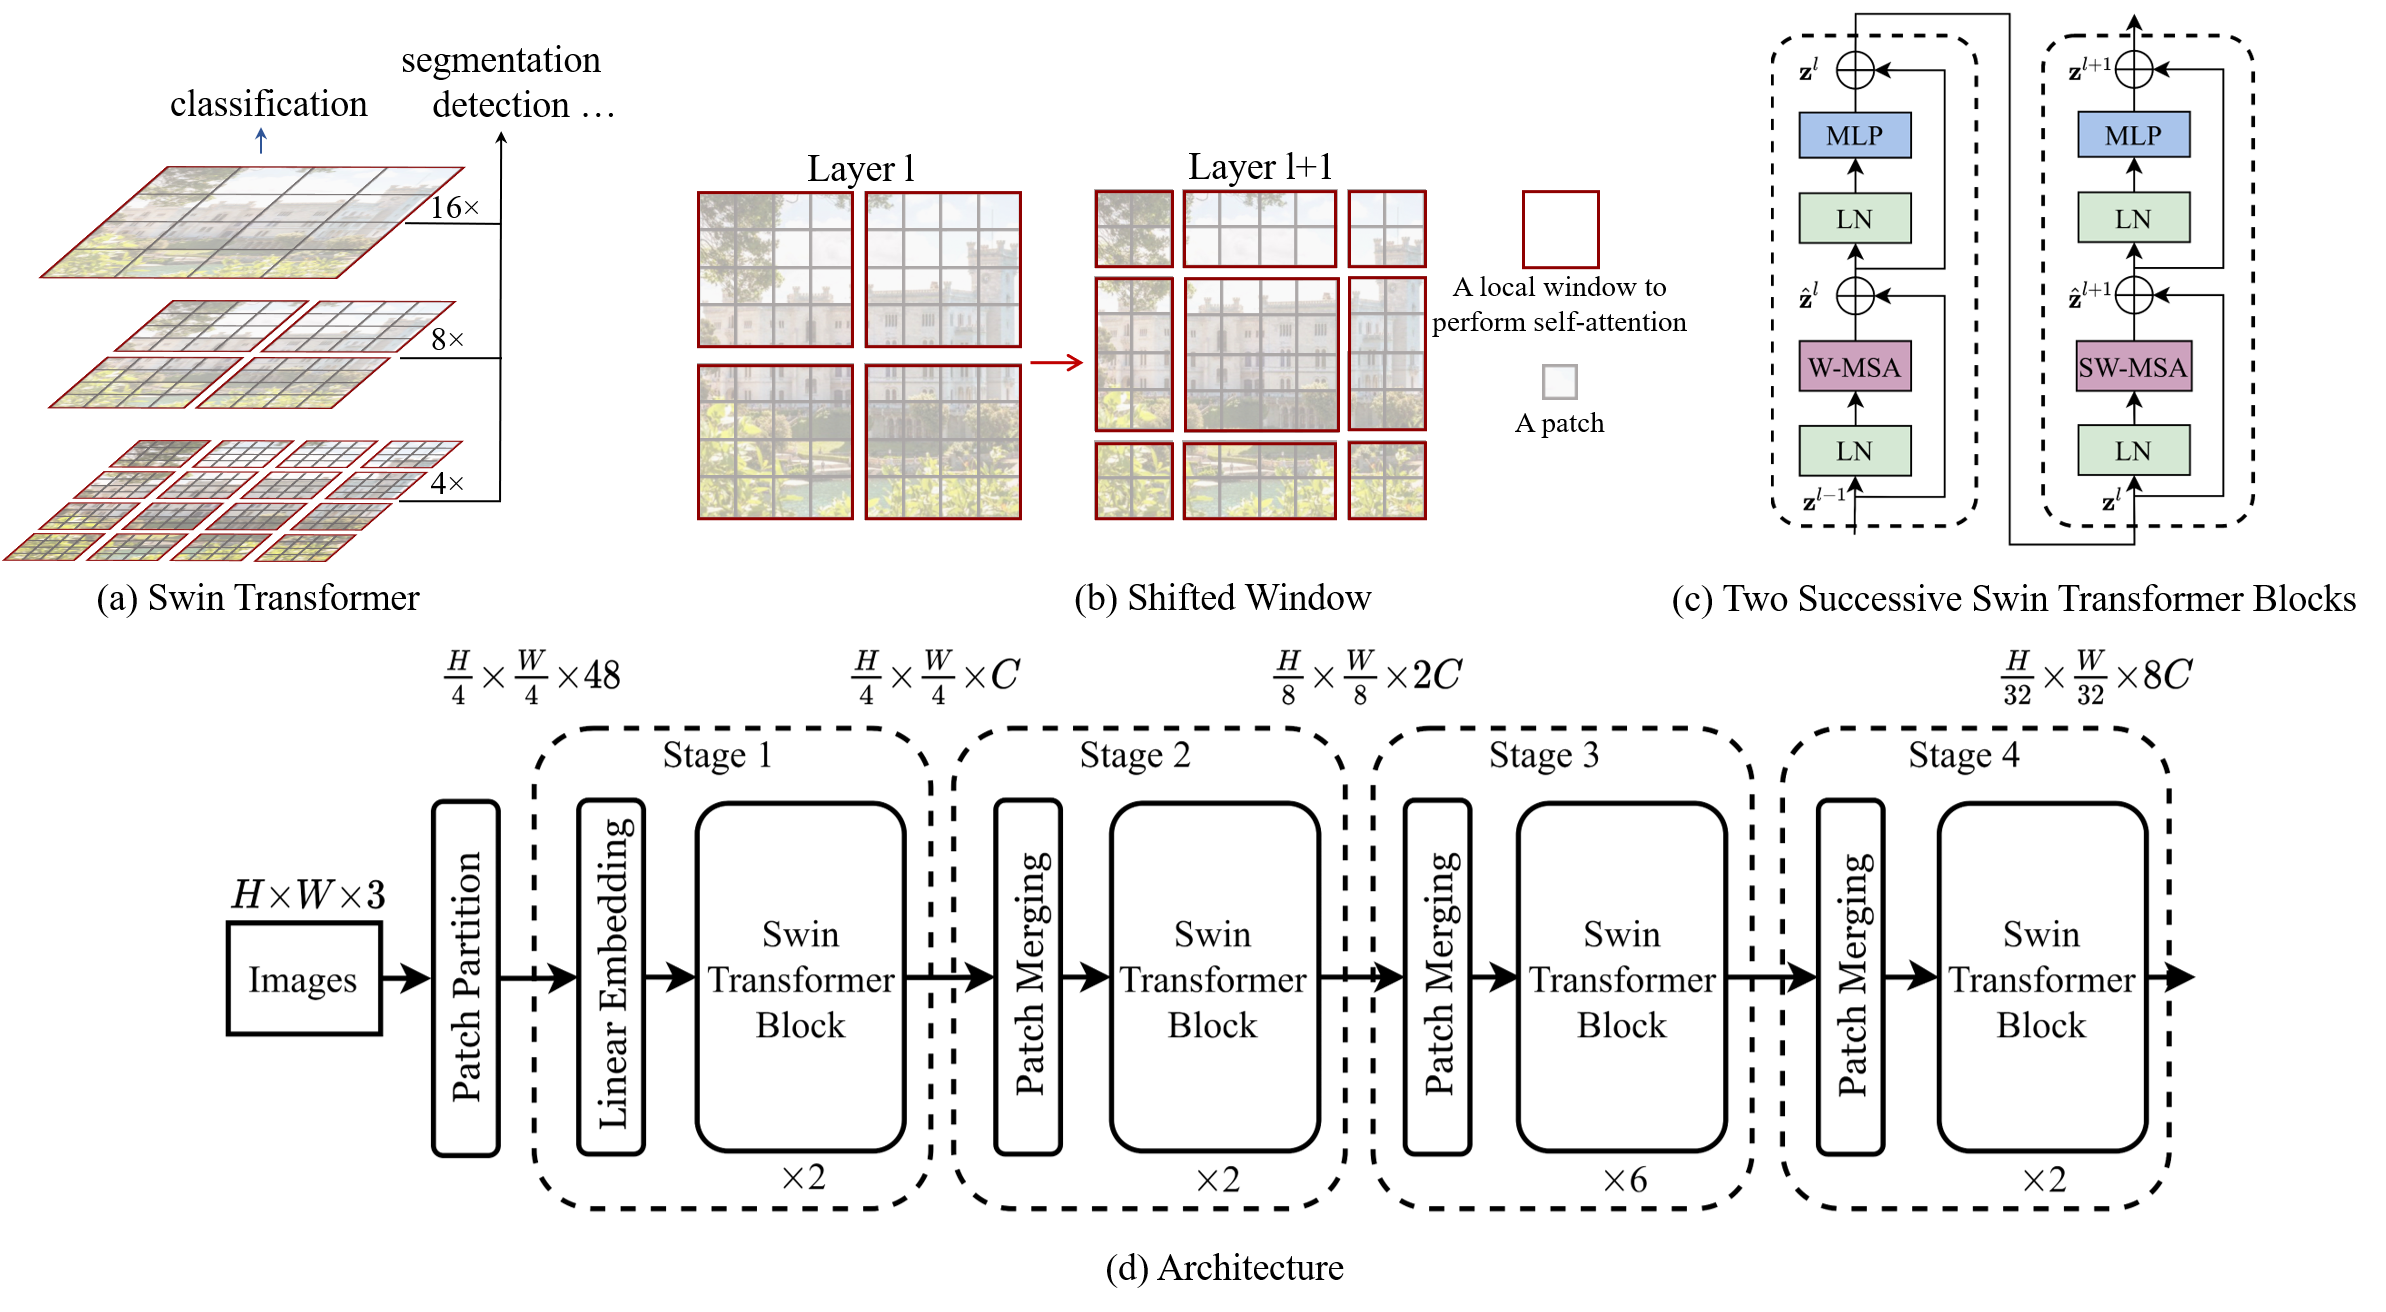
\includegraphics[width=0.8\textwidth]{Images/SwinTransformer.png}
  \caption{Swin Transformer components}
  \label{fig:swintransformer}
\end{figure}

\subsection{Final Architecture and pre-training}
The final architecture that has been proposed by Hatamizadeh et al. follows the
structure of U-Net3D, but in the encoder part, SwinTransformers are used instead
of the standard 3D Convolution. Some changes from the original paper have been
made in order to adapt the model to our type of data. From the original volume
of size $168 \times 280 \times 360$, we extract patches of size $96 \times 96
\times 96$. These patches are fed in the SwinUNetr model which is composed of a
4-stages Swin Transformer that acts as the encoder part and a sequence of
transposed convolutions as the decoder. For each stage of the encoder part, a
skip connection is added to the output of the decoder stage with the same shape,
as in the original U-Net architecture. The whole architecture is shown in Figure
\ref{fig:swinunetr}.

\begin{figure}[ht!]
  \centering
  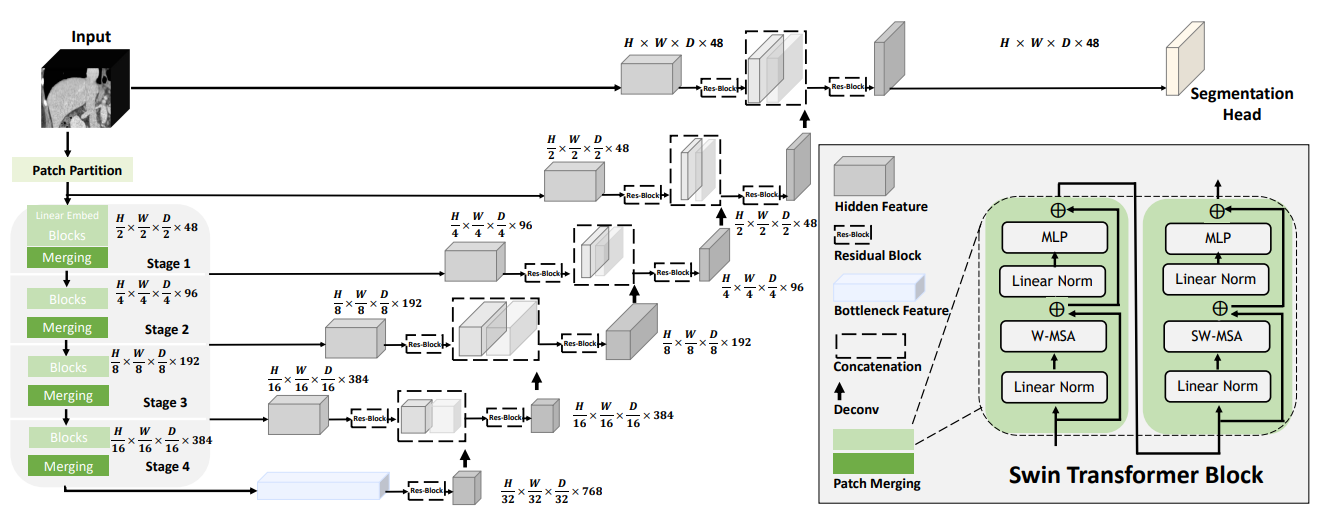
\includegraphics[width=0.8\textwidth]{Images/SwinUNETR.png}
  \caption{SwinUNETR architecture}
  \label{fig:swinunetr}
\end{figure}

As already mentioned, a pre-training phase is performed to overcome the data
hungriness characteristic of Transformers. The pretraining has been performed by
paper authors on a variety of datasets of CT scans of different types have been
used. A total of 5 public CT datasets, consisting of a total of 5,050 subjects,
are used to construct the pre-training dataset. We do not have tried to perform
the same pre-training on CBCT data instead of CT because the time required was
prohibitive.
The datasets used are:
\begin{itemize}
  \item{\textbf{Head \& Neck Squamous Cell Carcinoma (HNSCC)}: A collection
    contains imaging, radiation therapy, and clinical data from 627 head and
    neck squamous cell carcinoma (HNSCC) patients at MD Anderson Cancer Center.}
  \item{\textbf{Lung Nodule Analysis 2016 (LUNA 16)}: a collection of 888 CT
    scans of lung nodules.}
  \item{\textbf{TCIA CT Colonography Trial}: a collection of 825 CT colonography
    scans.}
  \item{\textbf{TCIA Covid 19}: a set of 2 datasets for a total of 753 CT scans
    of the chest and annotation about the Covid-19 infection.}
  \item{\textbf{TCIA LIDC-IDRI}: a collection obtained by the collaboration of
    seven academic centers and eight medical imaging companies. It contains 1018
    cases of diagnostic and lung cancer screening thoracic computed tomography
    (CT) scans with marked-up annotated lesions.}
\end{itemize}

\begin{figure}[ht!]
  \centering
  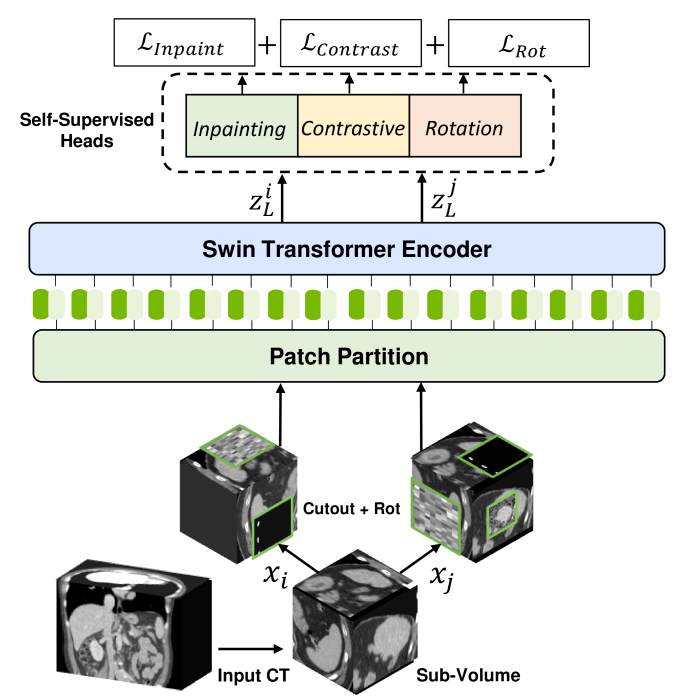
\includegraphics[width=0.4\textwidth]{Images/pretrain-unetr.png}
  \caption{Pre-training phase}
  \label{fig:pretrain-unetr}
\end{figure}
Multiple proxy tasks and formulated with a multi-objective loss function has
been used in that self-supervised phase:
\begin{itemize}
  \item{\textbf{Inpainting}: a transposed convolution layer have been attached
    to the encoder as reconstruction head, a patch is removed from the original
    volume and the model must manage to reconstruct the missing voxels, standard
    L1 loss $$\mathcal{L}_{inpaint} = ||\mathcal{X} - \hat{\mathcal{X}}||_1$$ is
    used, where $\hat{\mathcal{X}}$ is the output of the model and $\mathcal{X}$
    is the ground truth.}
  \item{\textbf{Image rotation}: The rotation prediction task predicts the angle
    categories by which the input sub-volume is rotated. For simplicity, we
    employ $R$ classes of $0$, $90$, $180$, and $270$ rotations along the
    z-axis. An MLP classification head is used for predicting the softmax
    probabilities $\hat{y}_r$ of rotation categories. Given the ground truth
    $y_r$, a cross-entropy loss is used for rotation prediction task:
    $$\mathcal{L}_{rot} = -\sum^R_{r=1}y_r\log(\hat{y}_r)$$}
  \item{\textbf{Contrastive coding}: The rotations used above where also used
    inside a contrastive loss. Given a batch of augmented sub-volumes, the
    contrastive coding allows for a better representation learning by maximizing
    the mutual information between positive pairs, while minimizing that between
    negative pairs. A linear layer is attached to the encoder to map each
    augmented sub.volume to a latent representation $v$. The cosing similarity
    is used as the distance measurement. The final loss between a pair $v_i$ and
    $v_j$ is defined as:
    $$\mathcal{L}_{contra} = -\log{\frac{\exp{(sim(v_i,v_j)/t)}}{\sum_k^{2N}1_{k
    \neq i}\exp{(sim(v_i,v_k)/t)}}}$$
    where $t$ is the measurement of normalized temperature scale. $1$ is the
    indicator function evaluating to $1 \iff k \neq i$, and $sim(\cdot, \cdot)$
    denotes the dot product between normalized embeddings.
    The contrastive learning loss function has been shown to strengthens the
    intra-class compactness as well as the inter-class separability.}
\end{itemize}

In conclusion, we minimize the final loss that is the sum of these 3 losses:
$$
\mathcal{L} = \lambda_1\mathcal{L}_{inpaint} + \lambda_2\mathcal{L}_{rot} +
\lambda_3\mathcal{L}_{contra}
$$
Where $\lambda_1$, $\lambda_2$ and $\lambda_3$ are the weights of the 3 losses
and are set to $1$ as experimentally shown to be the optimal value. In the
Figure \ref{fig:pretrain-unetr} this process is visually represented.

\section{Hann window function}
By looking at the whole segmented volume, we noticed that when using
PosPadUNet3D, the segmentation was not very accurate in the borders of each
patch. In order to solve this problem, we decided to extract overlapping patches
from the original volume instead of the non-overlapping method used in the
original paper. When two patches overlap, we would like to compute a weighted
average based on the distance from the center.
TODO: explain what happen in audio.
For this reason, we decided to apply the Hann window function to 3D volumes to
try to reduce edge effects.
\subsection{Hann window function in 1D}
The Hann window function, named after Julius von Hann, has been fist defined in
the field of signal processing, thus in 1D, as:
$$
w[n] = 0.5(1 - \cos(\frac{2\pi n}{N})), \quad n = 0, \dots, N
$$
where $x$ is the index of the window and $N$ is the total number of samples.
This function is symmetric, with a maximum value of $1$ in the middle of the
window and a minimum value of $0$ at the edges.
Another interesting property is that the sum of two Hann windows shifted by $\frac{N}{2}$
is equal to a rectangular window of width $N$ and height $1$:
\begin{equation}
  \label{eq:hannisone}
  w[n] + w[n + N] = 0.5(1 - \cos(\frac{2\pi n}{N})) + 0.5(1 - \cos(\frac{2\pi (n + N)}{N} )) = 1
\end{equation}
\subsection{Hann window function in 3D}
To apply the Hann window function in 3D, we simply apply the 1D function to each
dimension of the volume:
\begin{equation}
  w[x, y, z] = w[x]w[y]w[z]
\end{equation}
but we have to handle the case where the patch is close to the border of the
original volume. Here the patch is overlapped only on a part of the volume, thus
the window function must be adapted accordingly. In the 3D case, $27$ different
cases can occur, depending on the position of the patch in the original volume.
In Figure \ref{fig:hann-window} all the $9$ cases in the 2D scenario are shown.
Mathematically, this would require to define many different functions and being
unable to efficiently implement in Python the $N$-dimensional case, with $N$ as
a parameter.

% a 3x3 grid figure
\begin{figure}
  \centering
  \begin{subfigure}{0.5\textwidth}
    \centering
    %%%%%%%%%%%%
    \begin{subfigure}{.32\textwidth}
      \centering
      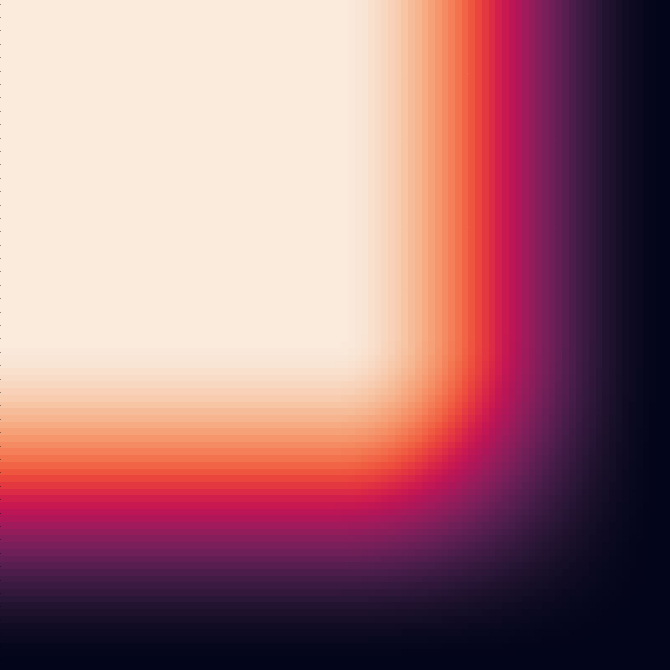
\includegraphics[width=\textwidth]{Images/hann_window_00.jpg}
    \end{subfigure}
    %%%%%%%%%%%
    \begin{subfigure}{.32\textwidth}
      \centering
      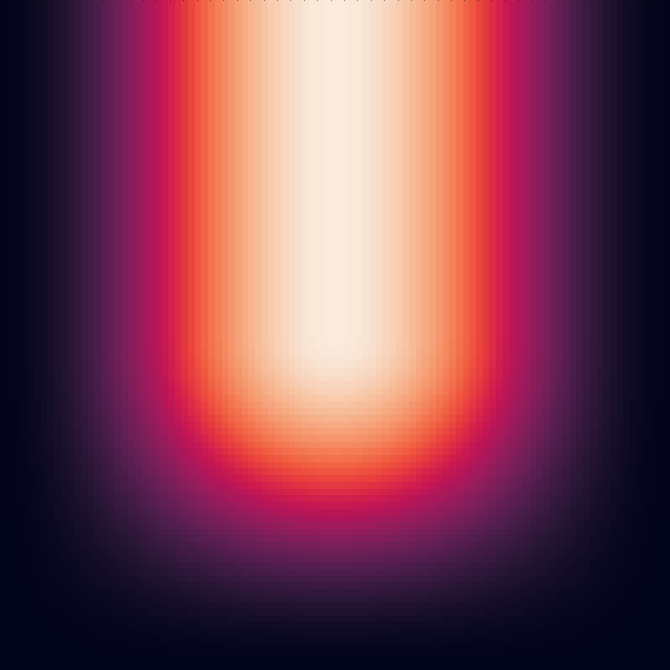
\includegraphics[width=\textwidth]{Images/hann_window_10.jpg}
    \end{subfigure}
    %%%%%%%%%%%
    \begin{subfigure}{.32\textwidth}
      \centering
      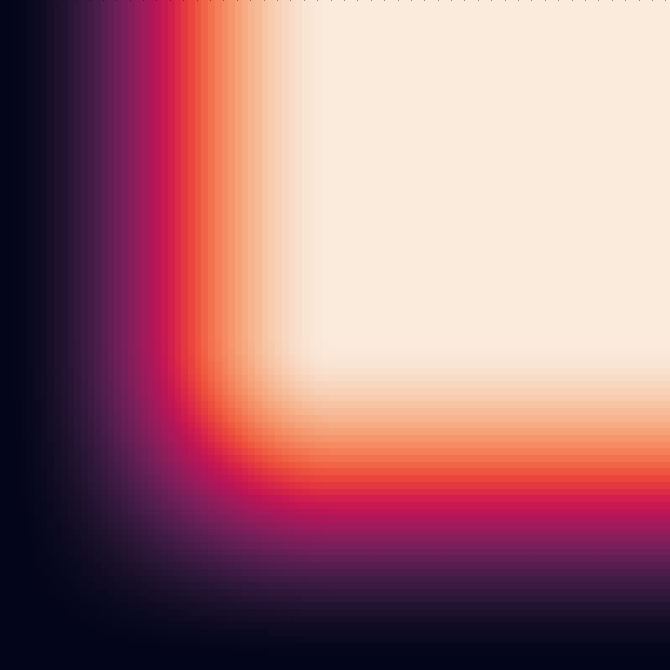
\includegraphics[width=\textwidth]{Images/hann_window_20.jpg}
    \end{subfigure}
    %%%%%%%%%%%
    \begin{subfigure}{.32\textwidth}
      \centering
      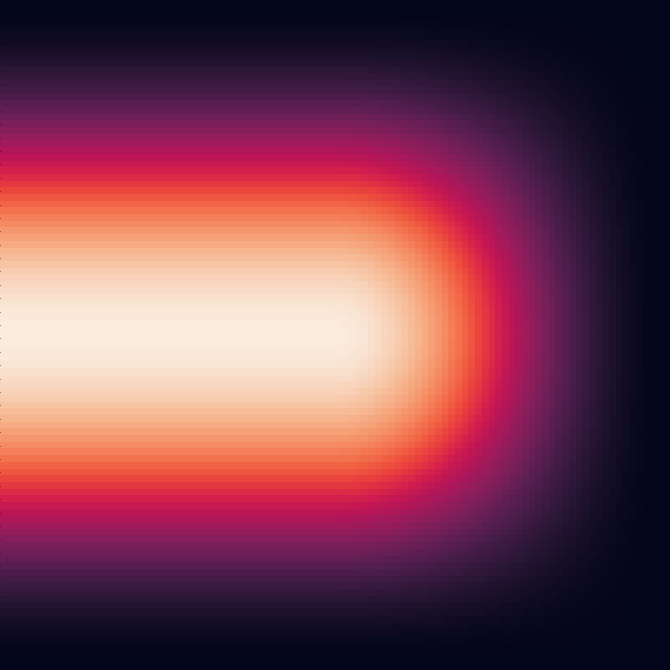
\includegraphics[width=\textwidth]{Images/hann_window_01.jpg}
    \end{subfigure}
    %%%%%%%%%%%
    \begin{subfigure}{.32\textwidth}
      \centering
      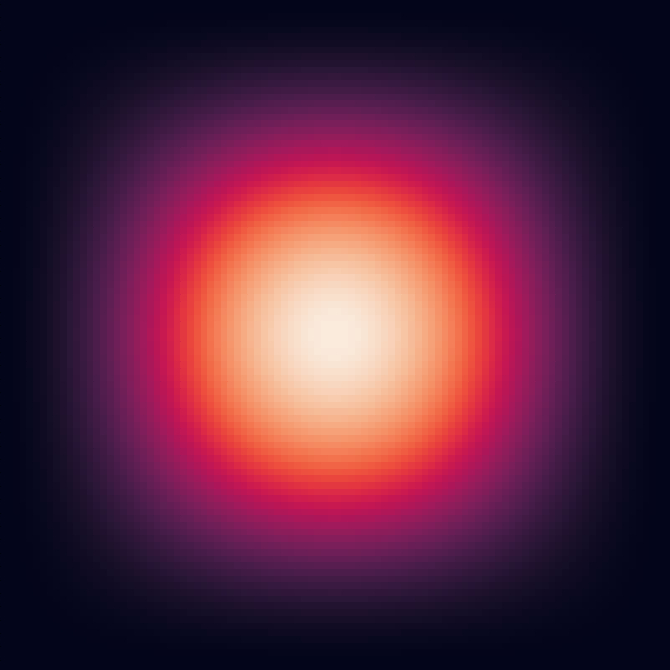
\includegraphics[width=\textwidth]{Images/hann_window_11.jpg}
    \end{subfigure}
    %%%%%%%%%%%
    \begin{subfigure}{.32\textwidth}
      \centering
      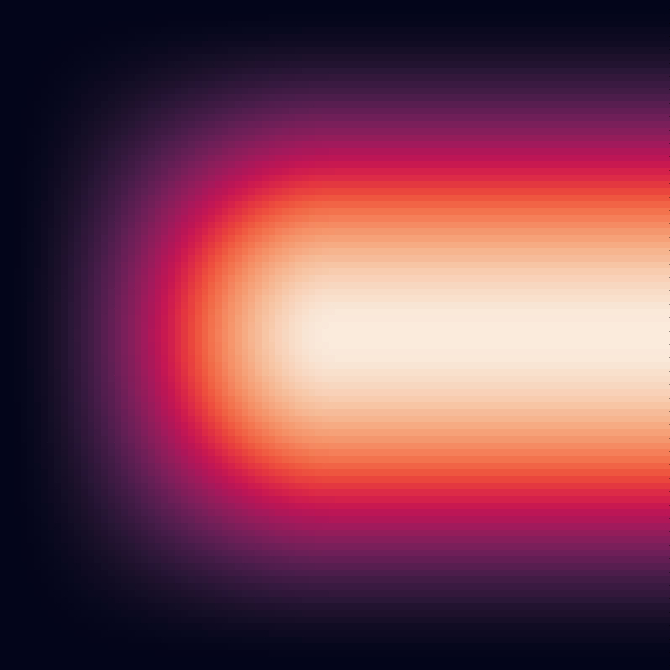
\includegraphics[width=\textwidth]{Images/hann_window_21.jpg}
    \end{subfigure}
    %%%%%%%%%%%
    \begin{subfigure}{.32\textwidth}
      \centering
      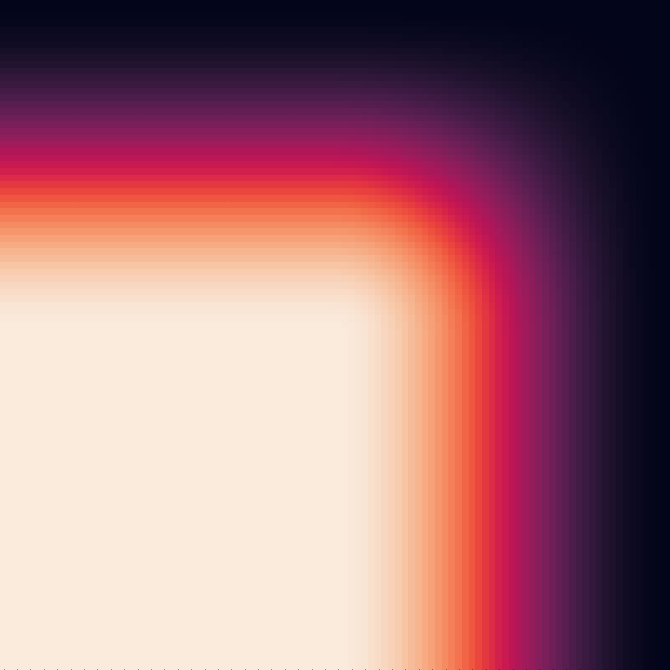
\includegraphics[width=\textwidth]{Images/hann_window_02.jpg}
    \end{subfigure}
    %%%%%%%%%%%
    \begin{subfigure}{.32\textwidth}
      \centering
      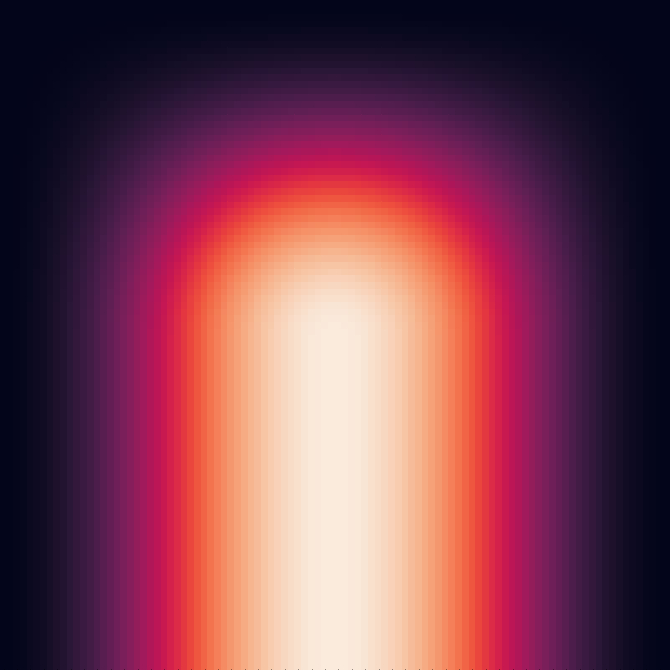
\includegraphics[width=\textwidth]{Images/hann_window_12.jpg}
    \end{subfigure}
    %%%%%%%%%%%
    \begin{subfigure}{.32\textwidth}
      \centering
      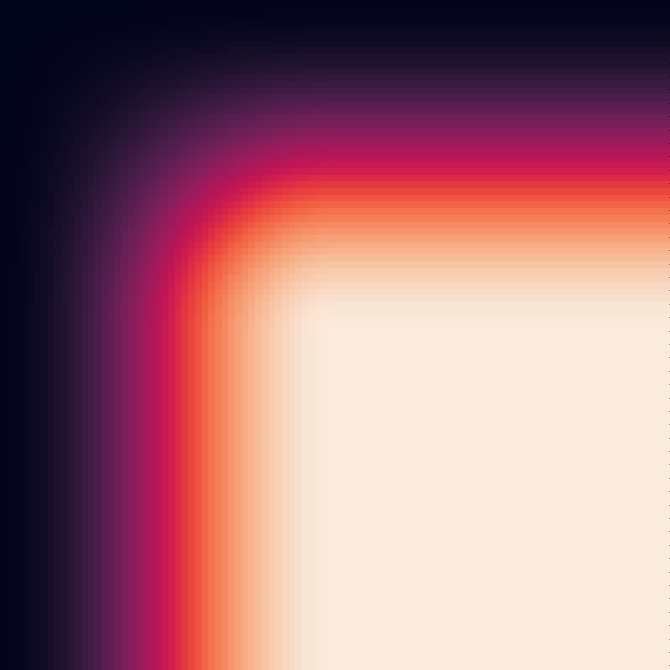
\includegraphics[width=\textwidth]{Images/hann_window_22.jpg}
    \end{subfigure}
  \end{subfigure}
  %%%%%%%%%%%
  \caption{Different Hann window functions in 2D based on the position of the extracted patch.}
  \label{fig:hann-window}
\end{figure}

\subsection{Implementation}
The first step is to generate a $N$-dim Hann window, by starting from a $1$-dim
window. Here we use the method provided in the PyTorch library \texttt{torch.hann\_window()}.
To produce a $2$-dim window, is possible to exploit the broadcast property of
tensors by multiplying a $1$-dim window with shape $(N,1)$
with a $1$-dim window with shape $(1,N)$, resulting in a $2$-dim window with
shape $(N,N)$. This process can be repeated to generate up to a $N$-dim window.
The code is shown in Listing \ref{alg:hann-window}. %Listing with title
\begin{lstlisting}[language=Python, caption=Python code to generate a $N$-dim Hann window, label=alg:hann-window]
def _get_hann_window(patch_size):
  hann_window_nd = torch.as_tensor([1])
  # create a n-dim hann window
  for spatial_dim, size in enumerate(patch_size):
    window_shape = np.ones_like(patch_size)
    window_shape[spatial_dim] = size
    hann_window_1d = torch.hann_window(
      size + 2,
      periodic=False,
    )
    hann_window_1d = hann_window_1d[1:-1].view(*window_shape)
    hann_window_nd = hann_window_nd * hann_window_1d
  return hann_window_nd
\end{lstlisting}

Once a $N$-dim Hann window is generated, the next step is to apply it to the
predicted segmnetation and, to avoid small numerical errors, we save the
coefficients used in a tensor of the same shape of the segmentation. These
numerical errors are due to the fact that these Hann windows are discrete and
not continuous, thus the sum of the window coefficients is not always equal to
$1$. Moreover this approach to avoid us to craft a specific window tensor for each
case near the border, which would become impratical for high dimensional cases.
The code is shown in Listing \ref{alg:apply-hann-window}.
\begin{lstlisting}[language=Python, caption=Code to apply Hann window to a batch of patches given their locations, label=alg:apply-hann-window]
hann_window = _get_hann_window(patch_size)
for patch, location in zip(batch, locations):
  i_ini, j_ini, k_ini, i_fin, j_fin, k_fin = location

  patch = patch * _hann_window
  _output_tensor[
      :,
      i_ini:i_fin,
      j_ini:j_fin,
      k_ini:k_fin,
  ] += patch
  _avgmask_tensor[
      :,
      i_ini:i_fin,
      j_ini:j_fin,
      k_ini:k_fin,
  ] += _hann_window
\end{lstlisting}

Once the segmentation for the whole volume is computed, the final step is to
divide the output tensor by the average mask tensor, to obtain the final
segmentation. The code is shown in Listing \ref{alg:final-segmentation}.

\begin{lstlisting}[language=Python, caption=Code to compute the final segmentation, label=alg:final-segmentation]
_output_tensor = _output_tensor / _avgmask_tensor
\end{lstlisting}

This method has been successfully implemented to TorchIO library and is avaible
since version $0.18.83$. The code is available at
\url{https://github.com/fepegar/torchio/blob/main/src/torchio/data/inference/aggregator.py}.

\section{Performance improvements}
The last attempt made aimed to improve the performance of the model without a
excessive drop in the metrics. Being that the face of a person is symmetrical,
we decided to crop each volume in two halves, and flip the right one, then we
trained the model on both halves separately. Moreover, as there is a considerable
space between the two halves, we managed to crop a little bit more of data
while leaving the canals still intact. We also wanted to be able to feed a single volume
into the network without having to extract smaller patches from it. To do so, we
resize the original volume by a factor of $3$. Once a resized volume is fed in
the network, we could resize them back to the original size and compute the
metrics as usual. With this approach, we managed to gain a speedup of $24$ times,
while the DICE score was only slightly affected by a drop of $0.02$.

\section{Results}
All the models have been trained using PyTorch, on two NVIDIA P100 GPUs with 16
GB of memory, over the AImagelab server.
The model proposed by Cipriano et al. achieved the best results among the
different tries and managed to keep the title of the state-of-the-art model for
the task of segmentation of the Inferior Alveolar Canal. However, the
experiments that have been made have obtained comparable metrics thus they might
open a new path to follow to improve such results.

% A table with 
